\subsection{Referencia de conectores}
A continuación presentamos una referencia a los conectores utilizados en los diagramas que se presentaran en las siguientes secciones. Los conectores \emph{no-standard} utlizados son especificados mas abajo.

\begin{multicols}{2}
\begin{figure}[H]
	\centering
	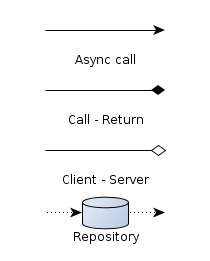
\includegraphics[scale=0.6]{graficos/call_reference.png}
	\caption{Referencia de conectores.}
\end{figure}
\begin{figure}[H]
  \centering
  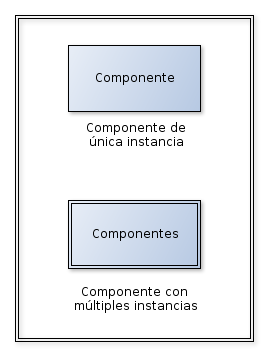
\includegraphics[scale=0.6]{graficos/comp_reference.png}
  \caption{Referencia de componentes.}
\end{figure}
\end{multicols}

\paragraph{Conectores no estandar}

\begin{itemize}
		%Completar con conectores no standard!
		%Agregar asi:
		\NonStandardConector{A non standard conector name}{A non standard conector description.}
\end{itemize}

\subsection{Conectividad external del sistema \textbf{TPA}}

En el siguiente diagrama vemos la disposición global del sistema central \textbf{TPA} respecto a los agentes externos con los que interactúa. 

\subsection{Subsistema de Query}

En el siguiente diagrama presenta el \textsf{Subsistema de Query} donde dada una consulta por productos (\textbf{query}) se arma la respuesta al usuario que realizó la consulta. En este diagrama se encuentran ejemplificados los \emph{casos de uso} 7, 8, 9, 10, 11 y 12.

\begin{figure}[H]
	\centering
	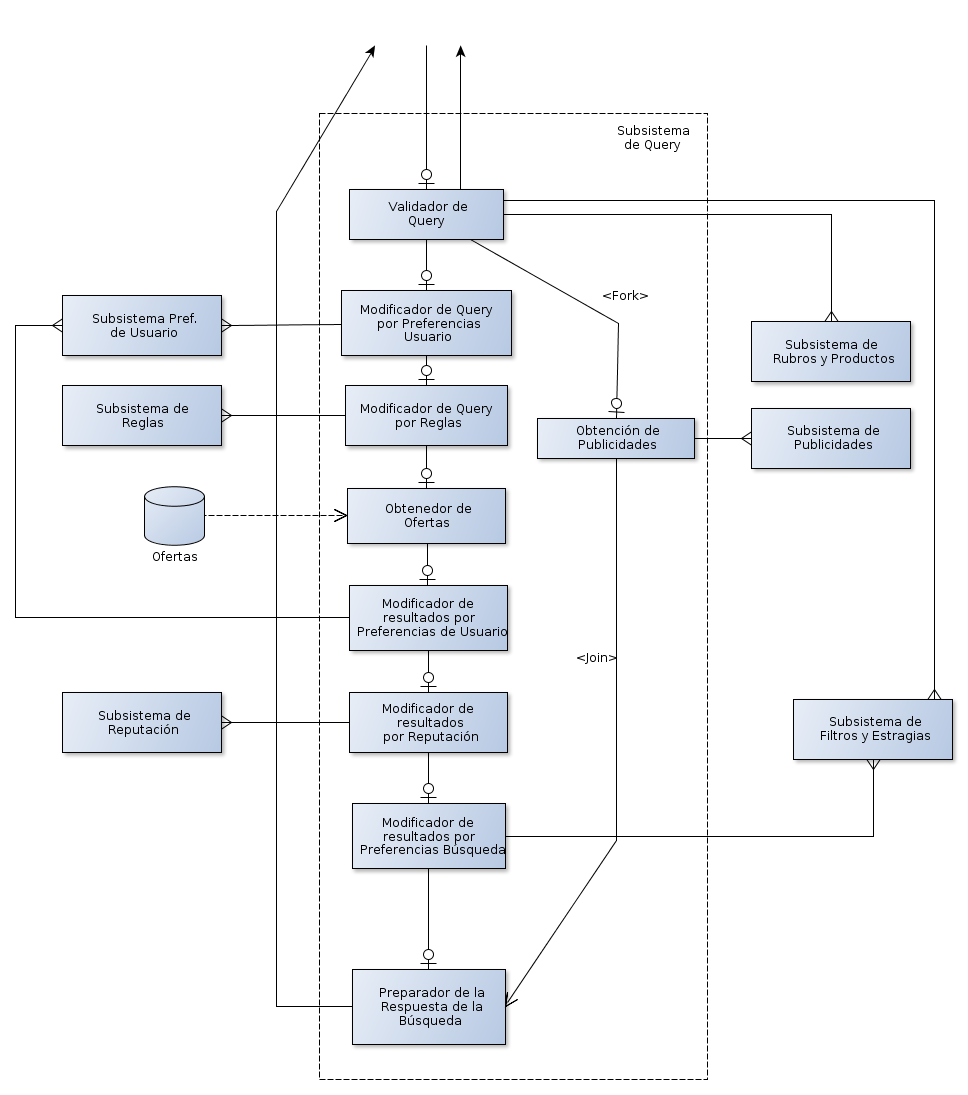
\includegraphics[width=\textwidth]{graficos/arch/subsistema_query.png}
	\caption{Diagrama arquitectónico con el detalle del \textsf{Subsistema de Query}.}
\end{figure}

La funcionalidad de este componente es la de procesar un pedido por productos para armar todo el contenido que le será devuelto al mismo. Este procesamiento incluye varias funcionalidades del sistema. Todas estas pueden realizarse de forma encadenada, lo cuál lleva a que el componente trabaje con un estilo arquitectónico de tipo \emph{pipe and filter}, en el cuál cada etapa de procesamiento se realiza secuencialmente pero de forma independiente. La elección de este estilo tiene como fin lograr \emph{modificabilidad} y \emph{performance}, ya que las etapas pueden reubicarse sin tener que modificar fuertemente el sistema, y para aquellas etapas que requieren mayor pueden agregarse más recursos, de forma que no generen un cuello de botella.

En primer lugar se valida que el pedido sea realizable (i.e.: es de un producto soportado y posee estrategias y filtros del sistema) por el \textsf{Validador de Query}. Dentro de las funcionalidades, se definieron distinas modificaciones que podrían sufrir las consultas. Los siguientes dos componentes (\textsf{Modificador de Query por Preferencias Usuario} y \textsf{Modificador de Query por Reglas}) se encargan de comunicarse con los subsistemas correspondientes que definen como debe realizarse las modificaciones. El validador encola la consulta para que sea procesada por estos componentes y a su vez la encola para que sea trabajada por el \textsf{Generador de publicidades}, que se encarga de generar las publicidades que formarán parte de la respuesta. Esto se realiza con un mecanismo de \emph{fork and join}, donde el \textsf{Generador de publicidades} toma la \emph{query}, la trabaja y luego espera a que sea consultado por el resultado. De esta forma, la generación de propagandas, que se considera independiente del resto del procesamiento a realizar, puede realizarse en paralelo, mejorando la \emph{performance del proceso}.

Las modificaciones que se realizan a la consulta están relacionadas con las preferencias del usuario (que puede decidir no ver las consultas provenientes de algunos usuarios) y las reglas de asociación y substitución, (que establecen que distintas extenciones a las búsquedas). La naturaleza de estas modificaciones no está completamente definida pero estará contenida exclusivamente en los \textsf{Subsistema de Preferencias de Usuario} y \textsf{Subsistema de Reglas}. 

Con la consulta (\emph{query}) ya definida y ajustada, el componente \textsf{Obtenedor de Ofertas} accede al repositorio de ofertas y adquiere todas aquellas que responden a la consulta.  Una vez realizado esto pasamos a la etapa donde se prepara el resultado. Por un lado el componente \textsf{Modificador de resultados por Preferencias de Usuario} se encarga de tareas como jerarquizar las ofertas según las preferencias del usuario. Las ofertas luego son decoradas, eliminadas y reorganizadas según la reputación de los usuarios que las originaron (componente \textsf{Modificador de resultados por Reputación}). A continuación se realiza un nuevo trabajo sobre los resultados aplicando los filtros y estrategias seleccionados por el usuario en la consulta original (componente \textsf{Modificador de resultados por filtros y estrategias}). Finalmente, el componente \textsf{Preparador de la Respuesta de la Búsqueda} prepara todo el paquete de respuesta que será enviado denuevo al usuario. 

\subsection{Interfáz movil}

\begin{figure}[H]
	\centering
	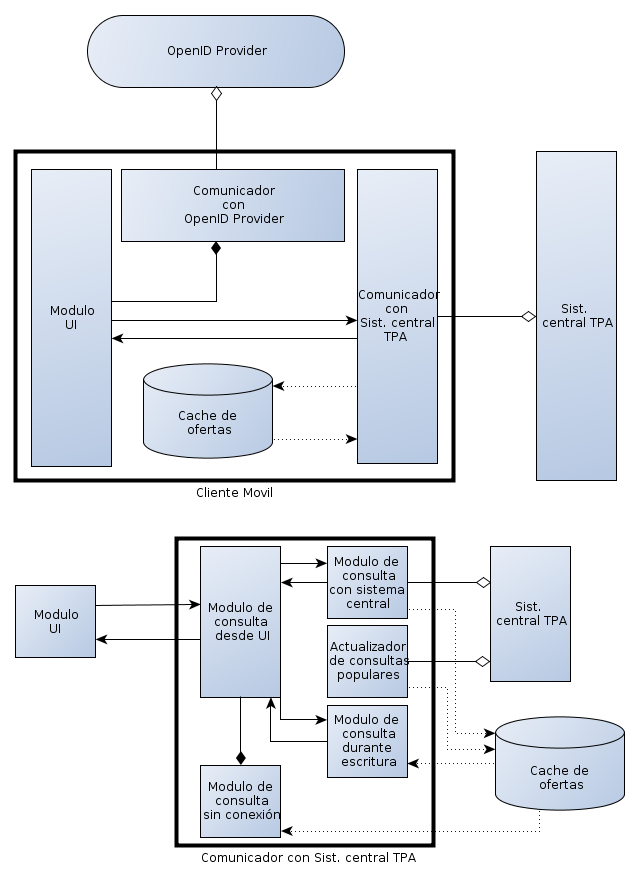
\includegraphics[width=\textwidth]{graficos/arch/Cliente_movil.png}
	\caption{Diagrama arquitectónico con el detalle del \textsf{Cliente movil}.}
\end{figure}

\subsection{Interfaz web}

\begin{figure}[H]
	\centering
	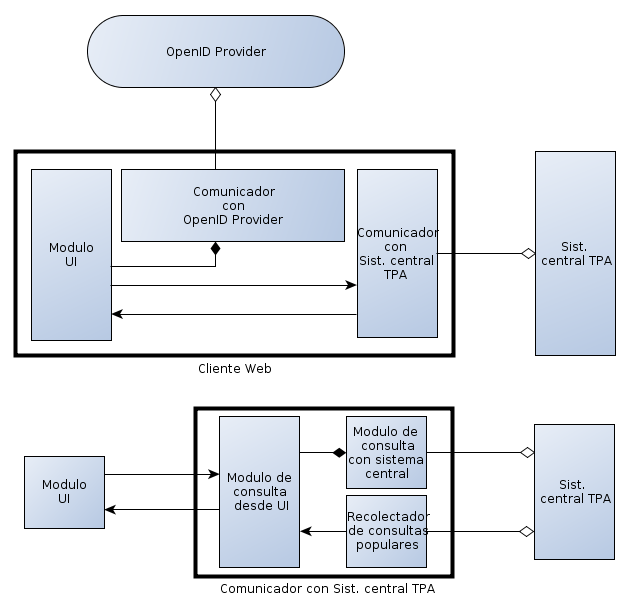
\includegraphics[width=\textwidth]{graficos/arch/Cliente_web.png}
	\caption{Diagrama arquitectónico con el detalle del \textsf{Cliente web}.}
\end{figure}
